\documentclass[a4paper,10pt]{article}

\usepackage[a4paper,left=1.0cm,right=1.0cm,top=2.0cm]{geometry}

\usepackage[utf8]{inputenc}
\usepackage{listings}
\usepackage{graphicx}
\usepackage[pdftex]{hyperref}
\usepackage{color}
\usepackage{textcomp}
\usepackage{float}

\definecolor{listinggray}{gray}{0.9}
\definecolor{lbcolor}{rgb}{0.9,0.9,0.9}

\lstset{
	backgroundcolor=\color{lbcolor},
	tabsize=2,
	rulecolor=,
	language=C,
        basicstyle=\scriptsize,
        upquote=true,
        aboveskip={1.5\baselineskip},
        columns=fixed,
        showstringspaces=false,
        extendedchars=true,
        breaklines=true,
        prebreak = \raisebox{0ex}[0ex][0ex]{\ensuremath{\hookleftarrow}},
        frame=single,
        showtabs=false,
        showspaces=false,
        showstringspaces=false,
        identifierstyle=\ttfamily,
        keywordstyle=\color[rgb]{0,0,1},
        commentstyle=\color[rgb]{0.133,0.545,0.133},
        stringstyle=\color[rgb]{0.627,0.126,0.941},
}

%opening
\title{4º Trabalho de Compiladores - Interpretador}
\author{André Siviero e Juan França}


\begin{document}

\maketitle

\begin{abstract}
Documentação referente à quarta parte do trabalho de compiladores, que consiste em um interpretador.
\end{abstract}

\section{Introdução}
O objetivo deste trabalho é estabelecer um interpretador para a linguagem PC (Poor C). Para construir esta parte, utiliza-se os três analisadores previamente construídos, ou seja,
os trabalhos anteriores foram incorporados nesta parte de tal forma que executar um programa checando erros sintáticos e semânticos da linguagem PC, exatamente como um interpretador faz.

\section{Menu}

Para facilitar a execução do código é criado um menu contendo as seguintes opções:

\begin{enumerate}
 \item Compilar um programa: construir a árvore de execução e ligá-la a uma struct s\_programa.
 \item Imprimir Árvore de Execução: basta imprimir cada nó da cmdList vasculhando também as árvores internas do nó
 \item Executar Programa: basta executar a cmdList de um Programa. 
 \item Listar programas compilados
 \item Listar programas no diretório corrente e subdiretórios (que podem ser compilados)
 \item Sair
\end{enumerate}

\section{Principais Estruturas}

Para criar e executar a árvore de execução é necessária a utilização de diversas estruturas. Cada estrutura segue a sua respectiva regra construída no segundo trabalho.
Cada estrutura possui a sua função de executar, normalmente, nomeada de \textbf{execute<estrutura>}. Por exemplo, para o fator, temos executeFator.

Segue abaixo a explicação sobre cada uma delas:

\subsection{Fator}
Esta é a mais baixa ordem da árvore. Pode ser inteiro, float, char, variável ou uma chamada de função. Sua estrutura é a seguinte:

\begin{lstlisting}
struct {
	int tipo;
	void *valor;
	list parametros;
} typedef s_fator;
\end{lstlisting}

A lista de parâmetros na chamada de função guarda os parâmetros passados pela função. É utilizada também para as atribuições ++/-- a variáveis. Um outro caso em que é utilizada,
é para explicitar que uma variável está com o valor negativo. 
O \textbf{tipo} serve para identificar qual typecast deve ser feito para capturar o valor correspondente a variável.\\
Esta manipulação é feita na função de execução. O caso de inteiro, char e float basta retornar o s\_fator correspondente. Porém, para a chamada de função e variável existem
considerações. O s\_fator a ser retornado nesse caso deve ser a versão avaliada destes fatores, isto é, o valor da variável ou o valor de retorno da função.
\subsection{Termo}

O termo fica um nível acima na árvore do Fator. É composta apenas por um sinal de operação que pode ser '*','/' e '\%'. Realiza operações sobre os fatores que estão abaixo dele na árvore.
No caso de não haver este nível na árvore, o Termo possuirá apenas um filho Fator, neste caso, a função executeTermo retornará este filho executado.

\begin{lstlisting}
 struct {
	char op;
} typedef s_termo
\end{lstlisting}

A função de execução do termo opera sobre os dois Fatores abaixo dele na árvore ou retorna a avaliação de seu único filho, quando for o caso. 
O operador aplicado sobre eles está na própria estrutura.

\subsection{EXP}
Basicamente, igual ao termo, porém os operadores são outros: '+','-'. Isto é feito para resolver o caso da precedência de operadores. Como a árvore é executada da folha para a raíza as operações de multiplicação, divisão e mod serão executadas primeiro do que as de soma e subtração.
No caso de não haver esse nível, a execução é tratada do mesmo modo que no Termo, sendo retornado o filho executado deste nó.

\begin{lstlisting}
struct {
	char op;
} typedef s_exp;
\end{lstlisting}

\subsection{U\_EXP}

Este é o caso em que os operadores: '>', '<', '>=' e '<=' foram inseridos. Assim pode-se comparar duas expressões e avaliar o valor.

\begin{lstlisting}
struct {
	char op[3];
} typedef s_u_exp;
\end{lstlisting}
Para facilitar a hierarquia das estruturas visualização segue uma figura:

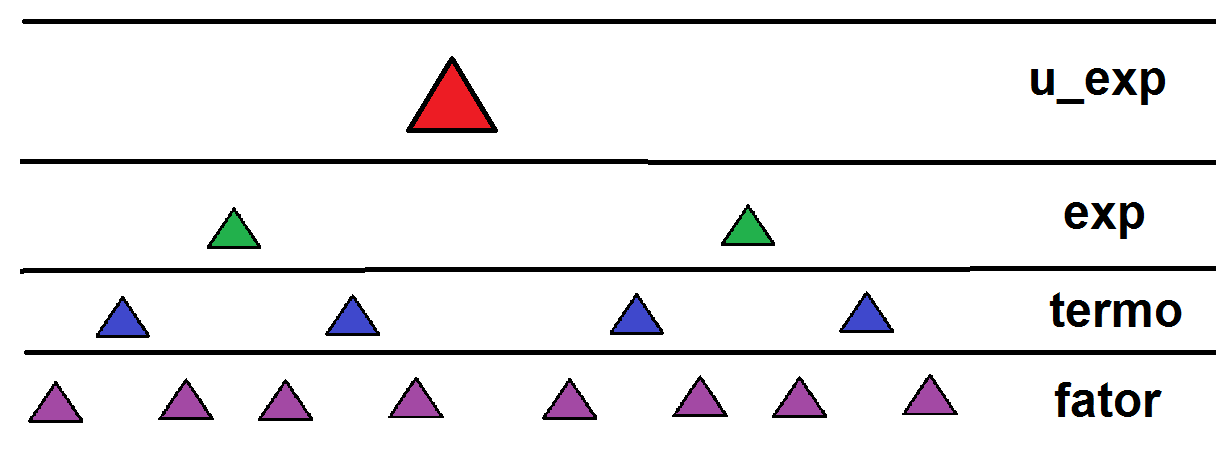
\includegraphics[scale=0.4]{figurinha.png}


\subsection{U\_Exp\_List}

É o conjunto de u\_exp e contém os operadores: '||', '\&\&' e '!=' para avaliar as u\_exp.

\begin{lstlisting}
struct {
	char op[2];
} typedef s_u_exp_list;
\end{lstlisting}

\subsection{Variable}

Estrutura reutilizada do terceiro trabalho para tratar as variáveis presentes no código. A sua estrutura é a seguinte:

\begin{lstlisting}
struct  {
  char nome[30];
  void *valor;
  int tipo;
  char escopo[30];
  int lineDeclared;
  int used;
} typedef s_variavel;
\end{lstlisting}
É bom distinguir que existe uma diferença entre a variável que esteja nesta forma da variável que está na forma de fator. Aqui, elas estão na
hashVar e possuem todos os dados disponíveis à disposição, enquanto que na forma de fator, apenas o nome e o tipo da variável são conhecidos. Assim,
quando uma variável estiver sendo executada, seu valor deve ser buscado na hash.
\subsection{Function}

Estrutura reutilizada do terceiro trabalho para tratar as funções presentes no código. A sua estrutura é a seguinte:

\begin{lstlisting}
struct  {
  char nome[30];
  int aridade;
  int tipo_retorno;
  list parametros;
  list parNames;
  list cmdList;
} typedef s_funcao;
\end{lstlisting}

Neste caso, foi inserido a lista cmdList que corresponde a uma lista de nós de árvore. Esta lista é utilizada para construção e execução da função.
\subsection{Atrib}

Referente as atribuições da linguagem C. 

\begin{lstlisting}
struct {
	char op[3];
	char varname[50];
	NODETREEPTR toatrib;
	char *stringToAtrib;
} typedef s_atrib;
\end{lstlisting}

Composta por um operador que pode ser '=','+=','-=','*=' e '/='. O nome da variável que receberá o valor do resultado da avaliação(feito pela função \textbf{executeNodeTree}) do nó toatrib. Foi criado o
stringToAtrib para o tipo string de dados, porém ele não foi implementado. 

\subsection{Conditional}

Correspondente aos comandos de seleção: if e else. A sua estrutura é a seguinte:

\begin{lstlisting}
struct {
	NODETREEPTR condition;
	list commandList;
	list elseCommandList;
} typedef s_conditional;
\end{lstlisting}

Composta pelo nó da condição e duas listas: execução do if e execução do else. Nem sempre estas listas estarão preenchidas, pois existem casos de Ifs
não-associados ou mesmo blocos vazios. A definição do tamanho dos blocos foi a maior dificuldade deste trabalho, especialmente nos casos em que havia
blocos e comandos aninhados, sendo muitas vezes a causa de Seg Faults difíceis de detectar. Implementamos uma espécie de pilha para isso, porém ela não é infalível. 

\subsection{Loop}

Correspondente aos loops permitidos na linguagem PC: for, while e do-while. A sua estrutura é a seguinte:

\begin{lstlisting}
struct {
	NODETREEPTR condition;
	list commandList;
	list atribList;
	list incrementList;
	int tipo;
} typedef s_loop;
\end{lstlisting}

Os comandos de repetição tem a condição e três listas: a de comandos, a de atribuição e a de incremento. O comando FOR por exemplo seria da forma:

\begin{lstlisting}
for ( atribList; condition; incrementList){
  commandList
}
\end{lstlisting}
Apenas um comando do tipo For possui a incrementList e a atribList, que são ``auxiliares'' em sua execução.
Na função de execução do comando de loop for basta executar primeiro a lista de atribuição, depois repetidamente checar a condição de parada, executar as listas de comandos e incremento, nesta ordem. 
No caso do while e \textbf{do while}, tem-se apenas que checar a condição de término do loop, lembrando que o \textbf{do while} deve executar ao menos
uma vez antes que as condições de parada sejam verificadas.

\subsection{Switch}

Para o switch utiliza-se a estrutura switch block que consiste em cada case referente ao respectivo switch. A lista de comandos é formada pelos ssb que possivelmente serão executados.
Cada switch possui o valor de check que será verificado com o valor do check do ssb. Como estabelicido no segundo trabalho, o switch deve obrigatoriamente ter um default para funcionar.

\begin{lstlisting}
struct switch_block{

    void* condition;
    list commands;
} typedef ssb;

struct {

	list commandList;
	char* check_value;
    char* check_value_s;

} typedef s_switch;
\end{lstlisting}

\subsection{Tree}
Corresponde a árvore genérica utilizada para . Cada nó corresponde a uma das estruturas acima mencionadas.
\begin{lstlisting}
struct nodeTree {
	void* element;
	struct nodeTree* next;
	list children;
	int tipoNodeTree;
};
\end{lstlisting}

Possui duas funções bem importantes: \textbf{executeNodeTree} e a \textbf{executeTreeList}. A primeira está exemplificada abaixo para demonstrar a recursividade. A segunda é simplesmente percorrer a lista executando a primeira função, verificando eventuais comandos de break, continue e return.

\begin{lstlisting}
s_fator *executeNodeTree(NODETREEPTR node) {
	s_fator *f,*r;
	s_variavel *v;
	switch(node->tipoNodeTree) {
		case F_FATOR:
			// Daqui pra baixo nao garanto nada
			f = (s_fator*)node->element;
			r = executaFator(f);

			if(f->tipo == T_VAR) {
				v = hashSearchVar(HashVar,(char*)f->valor,currentFunction);
				if(!v) {
					v = hashSearchVar(HashVar,(char*)f->valor,(char*)getNode(functionStack,functionStack->nElem-2));
				}

				if(f->parametros && f->parametros->head) {
					int *_t = getNode(f->parametros,0);
					if(*(int*)_t == P_MAISMAISAFT) {
						if(r->tipo == T_INT) {
							int _tmp = *(int*)r->valor + 1;
							*(int*)r->valor = _tmp;
						}
						else if(r->tipo == T_CHAR) {
							char _tmp = *(char*)r->valor + 1;
							*(char*)r->valor = _tmp;
						}
						else if(r->tipo == T_FLOAT) {
							float _tmp = *(float*)r->valor + 1;
							*(float*)r->valor = _tmp;
						}
					} else if(*(int*)_t == P_MENOSMENOSAFT) {
						if(r->tipo == T_INT) {
							int _tmp = *(int*)r->valor - 1;
							*(int*)r->valor = _tmp;
						}
						else if(v->tipo == T_CHAR) {
							char _tmp = *(char*)r->valor - 1;
							*(char*)r->valor = _tmp;
						}
						else if(r->tipo == T_FLOAT) {
							float _tmp = *(float*)r->valor - 1;
							*(float*)r->valor = _tmp;
						}
					}
				}
			}
			return r;
			break;
		case F_TERMO:
			return executeTermo((s_termo*)node->element,(list)(node->children->head->element));
			break;
		case F_EXP:
			return executeExp((s_exp*)node->element,(list)(node->children->head->element));
			break;
		case F_U_EXP:
			return executeU_Exp((s_u_exp*)node->element,(list)(node->children->head->element));
			break;
		case F_U_EXP_LIST:
			return executeU_Exp_List((s_u_exp_list*)node->element,(list)(node->children->head->element));
			break;
		case F_ATRIB:
			executeAtrib((s_atrib*)node->element,HashVar);
			return NULL;
			break;
		case F_CONDITIONAL:
			executeConditional((s_conditional*)node->element);
			return NULL;
			break;
		case F_LOOP:
		    executeLoop((s_loop*)node->element);
		    break;
		case F_RETURN:
			{
			break;} // LOL {} break :)
		case F_SWITCH:
		    executeSwitch((s_switch*)node->element);
		    break;
		default:
			break;

	}
	return NULL;
}
\end{lstlisting}

Observa-se que esta função atua como uma espécie de ``controlador'', gerenciando que função deve ser chamada pelo programa para executar um node. Isto
permite que ela seja usada em qualquer ponto do programa, desde que esteja atuando sobre nodetrees. Assim, o programa foi feito visando obter uma organização
em que os comandos sempre poderiam ser representados por árvores ou listas de árvores e a função a ser chamada para executar seria sempre a mesma, independente
do tipo de dados que se deve processar. Não é um exagero dizer que esta função é o ``cérebro'' do interpretador.
\section{cmdList}

Esta é a lista principal do programa. É composta por nós de árvore genéricos. Toda vez que um programa é executa a lista é percorrida executando todos as árvores, porém
seu comportamento pode ser alterado por flags de Break, Continue e Return. Estas flags foram definidas de maneira global para permitir que se propagassem
em cascata (especialmente o return, cujo efeito deve atingir toda a função).

\section{Programa}
Por fim, temos a estrutura de mais alto nível. A struct s\_programa contém uma commandList e suas hashes de função e variável. Cada novo programa redefine
as variaveis globais HashVar e HashFunc para montar sua struct de execução. Foi feito deste modo para que não fosse necessário modificar o código que já
estava pronto, porém atuava sobre um único programa principal. Após a compilação de um programa, o buffer do Bison é limpo e a variavel lines, zerada.
Caso a compilação tenha sido bem-sucedida, o programa é inserido na lista de programas do interpretador, podendo ser acessado pelo seu nome. Uma compilação
mal-sucedida gera um erro e o usuário é remetido de volta ao menu.

Para a execução, o programa precisa apontar os ponteiros globais HashVar e HashFunc para suas proprias Hashes, evitando a situação de um programa
ter acesso a variáveis e funções de outro já compilado, ao mesmo tempo em que diz ao interpretador quais variáveis estão disponíveis.

\section{Funções Nativas}
Existem algumas funções pré-definidas na linguagem. Estas podem ser usadas para melhor codificação na linguagem PC.
\subsection{printf}
Assim como em C, na PC existe uma função para imprimir dados na tela. Esta função possui aridade 2 e aceita a dados inteiros(\%d), float(\%f) e char (\%c). Nos exemplos,
pode-se ver vários exemplos de uso. Como a aridade de printf é fixa, sempre que se quiser imprimir apenas uma string, deve-se usar um parametro dummy como
segundo parâmetro. Isto foi demonstrado nos exemplos.
\subsection{scanf}
Assim como em C, também é necessário uma função para entrada de dados. Porém, na PC existe uma diferença. Para indicar a variável em que será inserido o valor não é preciso 
utilizar o \& para indiciar o endereço da variável, basta inserir o nome da variável normalmente.
\subsection{max}
Essa função retorna o maior valor entre dois inteiros, dois float ou dois chars. Existe a restrição de tipos, ou seja, não é permitido passar como parâmetro um inteiro e um float. Apenas inteiro com inteiro, e assim sucessivamente.
\subsection{min}
Análoga à função acima, com a diferença de que o retorno é o valor mínimo entre as variáveis.
\section{Exemplos}

Nos exemplos, exploramos diversas situações para os diversos tipos de usuários. Foram criadas 10 situações, 5 situações corretas e 5 
situações erradas.
\end{document}